\documentclass[]{article}
\usepackage{lmodern}
\usepackage{amssymb,amsmath}
\usepackage{ifxetex,ifluatex}
\usepackage{fixltx2e} % provides \textsubscript
\ifnum 0\ifxetex 1\fi\ifluatex 1\fi=0 % if pdftex
  \usepackage[T1]{fontenc}
  \usepackage[utf8]{inputenc}
\else % if luatex or xelatex
  \ifxetex
    \usepackage{mathspec}
  \else
    \usepackage{fontspec}
  \fi
  \defaultfontfeatures{Ligatures=TeX,Scale=MatchLowercase}
\fi
% use upquote if available, for straight quotes in verbatim environments
\IfFileExists{upquote.sty}{\usepackage{upquote}}{}
% use microtype if available
\IfFileExists{microtype.sty}{%
\usepackage{microtype}
\UseMicrotypeSet[protrusion]{basicmath} % disable protrusion for tt fonts
}{}
\usepackage[margin=1in]{geometry}
\usepackage{hyperref}
\hypersetup{unicode=true,
            pdftitle={MEGAHAND},
            pdfauthor={Joe},
            pdfborder={0 0 0},
            breaklinks=true}
\urlstyle{same}  % don't use monospace font for urls
\usepackage{color}
\usepackage{fancyvrb}
\newcommand{\VerbBar}{|}
\newcommand{\VERB}{\Verb[commandchars=\\\{\}]}
\DefineVerbatimEnvironment{Highlighting}{Verbatim}{commandchars=\\\{\}}
% Add ',fontsize=\small' for more characters per line
\usepackage{framed}
\definecolor{shadecolor}{RGB}{248,248,248}
\newenvironment{Shaded}{\begin{snugshade}}{\end{snugshade}}
\newcommand{\KeywordTok}[1]{\textcolor[rgb]{0.13,0.29,0.53}{\textbf{#1}}}
\newcommand{\DataTypeTok}[1]{\textcolor[rgb]{0.13,0.29,0.53}{#1}}
\newcommand{\DecValTok}[1]{\textcolor[rgb]{0.00,0.00,0.81}{#1}}
\newcommand{\BaseNTok}[1]{\textcolor[rgb]{0.00,0.00,0.81}{#1}}
\newcommand{\FloatTok}[1]{\textcolor[rgb]{0.00,0.00,0.81}{#1}}
\newcommand{\ConstantTok}[1]{\textcolor[rgb]{0.00,0.00,0.00}{#1}}
\newcommand{\CharTok}[1]{\textcolor[rgb]{0.31,0.60,0.02}{#1}}
\newcommand{\SpecialCharTok}[1]{\textcolor[rgb]{0.00,0.00,0.00}{#1}}
\newcommand{\StringTok}[1]{\textcolor[rgb]{0.31,0.60,0.02}{#1}}
\newcommand{\VerbatimStringTok}[1]{\textcolor[rgb]{0.31,0.60,0.02}{#1}}
\newcommand{\SpecialStringTok}[1]{\textcolor[rgb]{0.31,0.60,0.02}{#1}}
\newcommand{\ImportTok}[1]{#1}
\newcommand{\CommentTok}[1]{\textcolor[rgb]{0.56,0.35,0.01}{\textit{#1}}}
\newcommand{\DocumentationTok}[1]{\textcolor[rgb]{0.56,0.35,0.01}{\textbf{\textit{#1}}}}
\newcommand{\AnnotationTok}[1]{\textcolor[rgb]{0.56,0.35,0.01}{\textbf{\textit{#1}}}}
\newcommand{\CommentVarTok}[1]{\textcolor[rgb]{0.56,0.35,0.01}{\textbf{\textit{#1}}}}
\newcommand{\OtherTok}[1]{\textcolor[rgb]{0.56,0.35,0.01}{#1}}
\newcommand{\FunctionTok}[1]{\textcolor[rgb]{0.00,0.00,0.00}{#1}}
\newcommand{\VariableTok}[1]{\textcolor[rgb]{0.00,0.00,0.00}{#1}}
\newcommand{\ControlFlowTok}[1]{\textcolor[rgb]{0.13,0.29,0.53}{\textbf{#1}}}
\newcommand{\OperatorTok}[1]{\textcolor[rgb]{0.81,0.36,0.00}{\textbf{#1}}}
\newcommand{\BuiltInTok}[1]{#1}
\newcommand{\ExtensionTok}[1]{#1}
\newcommand{\PreprocessorTok}[1]{\textcolor[rgb]{0.56,0.35,0.01}{\textit{#1}}}
\newcommand{\AttributeTok}[1]{\textcolor[rgb]{0.77,0.63,0.00}{#1}}
\newcommand{\RegionMarkerTok}[1]{#1}
\newcommand{\InformationTok}[1]{\textcolor[rgb]{0.56,0.35,0.01}{\textbf{\textit{#1}}}}
\newcommand{\WarningTok}[1]{\textcolor[rgb]{0.56,0.35,0.01}{\textbf{\textit{#1}}}}
\newcommand{\AlertTok}[1]{\textcolor[rgb]{0.94,0.16,0.16}{#1}}
\newcommand{\ErrorTok}[1]{\textcolor[rgb]{0.64,0.00,0.00}{\textbf{#1}}}
\newcommand{\NormalTok}[1]{#1}
\usepackage{graphicx,grffile}
\makeatletter
\def\maxwidth{\ifdim\Gin@nat@width>\linewidth\linewidth\else\Gin@nat@width\fi}
\def\maxheight{\ifdim\Gin@nat@height>\textheight\textheight\else\Gin@nat@height\fi}
\makeatother
% Scale images if necessary, so that they will not overflow the page
% margins by default, and it is still possible to overwrite the defaults
% using explicit options in \includegraphics[width, height, ...]{}
\setkeys{Gin}{width=\maxwidth,height=\maxheight,keepaspectratio}
\IfFileExists{parskip.sty}{%
\usepackage{parskip}
}{% else
\setlength{\parindent}{0pt}
\setlength{\parskip}{6pt plus 2pt minus 1pt}
}
\setlength{\emergencystretch}{3em}  % prevent overfull lines
\providecommand{\tightlist}{%
  \setlength{\itemsep}{0pt}\setlength{\parskip}{0pt}}
\setcounter{secnumdepth}{0}
% Redefines (sub)paragraphs to behave more like sections
\ifx\paragraph\undefined\else
\let\oldparagraph\paragraph
\renewcommand{\paragraph}[1]{\oldparagraph{#1}\mbox{}}
\fi
\ifx\subparagraph\undefined\else
\let\oldsubparagraph\subparagraph
\renewcommand{\subparagraph}[1]{\oldsubparagraph{#1}\mbox{}}
\fi

%%% Use protect on footnotes to avoid problems with footnotes in titles
\let\rmarkdownfootnote\footnote%
\def\footnote{\protect\rmarkdownfootnote}

%%% Change title format to be more compact
\usepackage{titling}

% Create subtitle command for use in maketitle
\newcommand{\subtitle}[1]{
  \posttitle{
    \begin{center}\large#1\end{center}
    }
}

\setlength{\droptitle}{-2em}

  \title{MEGAHAND}
    \pretitle{\vspace{\droptitle}\centering\huge}
  \posttitle{\par}
    \author{Joe}
    \preauthor{\centering\large\emph}
  \postauthor{\par}
      \predate{\centering\large\emph}
  \postdate{\par}
    \date{11/8/2018}


\begin{document}
\maketitle

\section{Interoperability}\label{interoperability}

\begin{Shaded}
\begin{Highlighting}[]
\CommentTok{# install.packages("tidyverse")}
\KeywordTok{library}\NormalTok{(tidyverse)}
\end{Highlighting}
\end{Shaded}

\begin{verbatim}
## -- Attaching packages ------------------------------------------------------------------ tidyverse 1.2.1 --
\end{verbatim}

\begin{verbatim}
## v ggplot2 3.0.0     v purrr   0.2.5
## v tibble  1.4.2     v dplyr   0.7.6
## v tidyr   0.8.1     v stringr 1.3.1
## v readr   1.1.1     v forcats 0.3.0
\end{verbatim}

\begin{verbatim}
## -- Conflicts --------------------------------------------------------------------- tidyverse_conflicts() --
## x dplyr::filter() masks stats::filter()
## x dplyr::lag()    masks stats::lag()
\end{verbatim}

\begin{Shaded}
\begin{Highlighting}[]
\CommentTok{# install.packages("reticulate", dependencies = TRUE)}
\KeywordTok{library}\NormalTok{(reticulate)}
\end{Highlighting}
\end{Shaded}

With the reticulate package in R, Python code can be integrated into R
documents and used alongside R. This is especially convenient in the
RMarkdown document format for several reasons:

\begin{itemize}
\item
  R code and Python code can be called in discrete boxes, but within the
  same document
\item
  Objects built in either environment can be passed back and forth
  between languages
\item
  RMarkdown offers flexible export formats including pdf, slides, word,
  and html
\end{itemize}

This particular aspect of our project interested me due to the scale and
diversity of challenges in interoperability.

\begin{Shaded}
\begin{Highlighting}[]
\ImportTok{import}\NormalTok{ numpy }\ImportTok{as}\NormalTok{ np}
\ImportTok{import}\NormalTok{ pandas }\ImportTok{as}\NormalTok{ pd}
\ImportTok{import}\NormalTok{ matplotlib.pyplot }\ImportTok{as}\NormalTok{ plt}
\end{Highlighting}
\end{Shaded}

\section{Exploratory Data Analysis and
Visualization}\label{exploratory-data-analysis-and-visualization}

This is a Python script that grabs all of the ``.csv'' files in a
folder, and makes a list of the names. The script is saved as
``TrainingDataGrabber.py''

\begin{Shaded}
\begin{Highlighting}[]
\ImportTok{import}\NormalTok{ os}
\ImportTok{import}\NormalTok{ glob}
\NormalTok{path }\OperatorTok{=} \StringTok{'c:}\CharTok{\textbackslash{}\textbackslash{}}\StringTok{'}
\NormalTok{extension }\OperatorTok{=} \StringTok{'csv'}
\NormalTok{os.chdir(path}\OperatorTok{=} \StringTok{"C:/Users/joeje/Desktop/Academics/FAES/Intro_to_Python/MEGAHAND/TrainingData"}\NormalTok{)}
\NormalTok{Training_Data_Files }\OperatorTok{=}\NormalTok{ [i }\ControlFlowTok{for}\NormalTok{ i }\KeywordTok{in}\NormalTok{ glob.glob(}\StringTok{'*.}\SpecialCharTok{\{\}}\StringTok{'}\NormalTok{.}\BuiltInTok{format}\NormalTok{(extension))]}
\BuiltInTok{print}\NormalTok{(Training_Data_Files)}
\end{Highlighting}
\end{Shaded}

Here, I used R to source the Python script, create a list object
containing all of the file names in the ``TrainingData'' folder, and
then coerced an R DataFrame from that list for display.

\begin{Shaded}
\begin{Highlighting}[]
\NormalTok{reticulate}\OperatorTok{::}\KeywordTok{source_python}\NormalTok{(}\StringTok{"TrainingDataGrabber.py"}\NormalTok{)}

\NormalTok{Training_Data_Files}
\end{Highlighting}
\end{Shaded}

\begin{verbatim}
##  [1] "Chuck Grip.csv"     "Fine Pinch.csv"     "H. Open.csv"       
##  [4] "Hook Grip.csv"      "Key Grip.csv"       "No Move.csv"       
##  [7] "Power Grip.csv"     "Thumb Enclosed.csv" "Tool Grip.csv"     
## [10] "W. Abduction.csv"   "W. Adduction.csv"   "W. Extension.csv"  
## [13] "W. Flexion.csv"     "W. Pronation.csv"   "W. Supination.csv"
\end{verbatim}

\begin{Shaded}
\begin{Highlighting}[]
\KeywordTok{as.data.frame}\NormalTok{(Training_Data_Files)}
\end{Highlighting}
\end{Shaded}

\begin{verbatim}
##    Training_Data_Files
## 1       Chuck Grip.csv
## 2       Fine Pinch.csv
## 3          H. Open.csv
## 4        Hook Grip.csv
## 5         Key Grip.csv
## 6          No Move.csv
## 7       Power Grip.csv
## 8   Thumb Enclosed.csv
## 9        Tool Grip.csv
## 10    W. Abduction.csv
## 11    W. Adduction.csv
## 12    W. Extension.csv
## 13      W. Flexion.csv
## 14    W. Pronation.csv
## 15   W. Supination.csv
\end{verbatim}

Next, I used the purrr package from R to apply a function I made in R
that tidys the data (removing extraneous columns and formatting) and
then creates a pre-set visualization for all of the files from the list
(that was made in Python.)

\begin{Shaded}
\begin{Highlighting}[]
\KeywordTok{source}\NormalTok{(}\StringTok{"C:/Users/joeje/Desktop/Academics/FAES/Intro_to_Python/MEGAHAND/Megamunge_Jitter.R"}\NormalTok{)}
\KeywordTok{library}\NormalTok{(purrr)}
\KeywordTok{setwd}\NormalTok{(}\StringTok{'TrainingData'}\NormalTok{)}
\KeywordTok{map}\NormalTok{(Training_Data_Files, Megamunge)}
\end{Highlighting}
\end{Shaded}

\begin{verbatim}
## [[1]]
\end{verbatim}

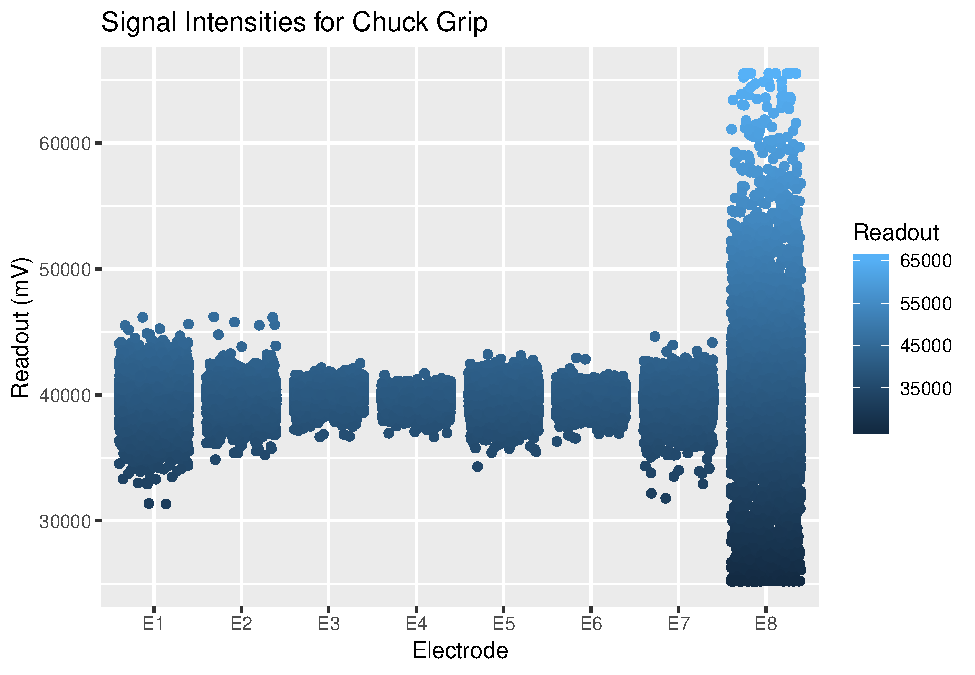
\includegraphics{Megahand_files/figure-latex/unnamed-chunk-5-1.pdf}

\begin{verbatim}
## 
## [[2]]
\end{verbatim}

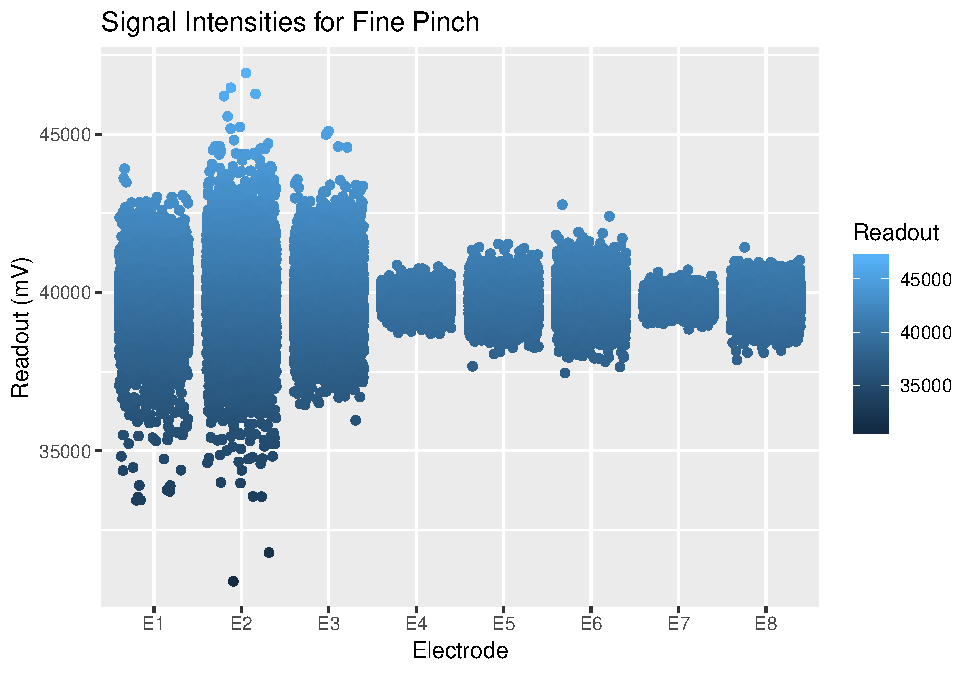
\includegraphics{Megahand_files/figure-latex/unnamed-chunk-5-2.pdf}

\begin{verbatim}
## 
## [[3]]
\end{verbatim}

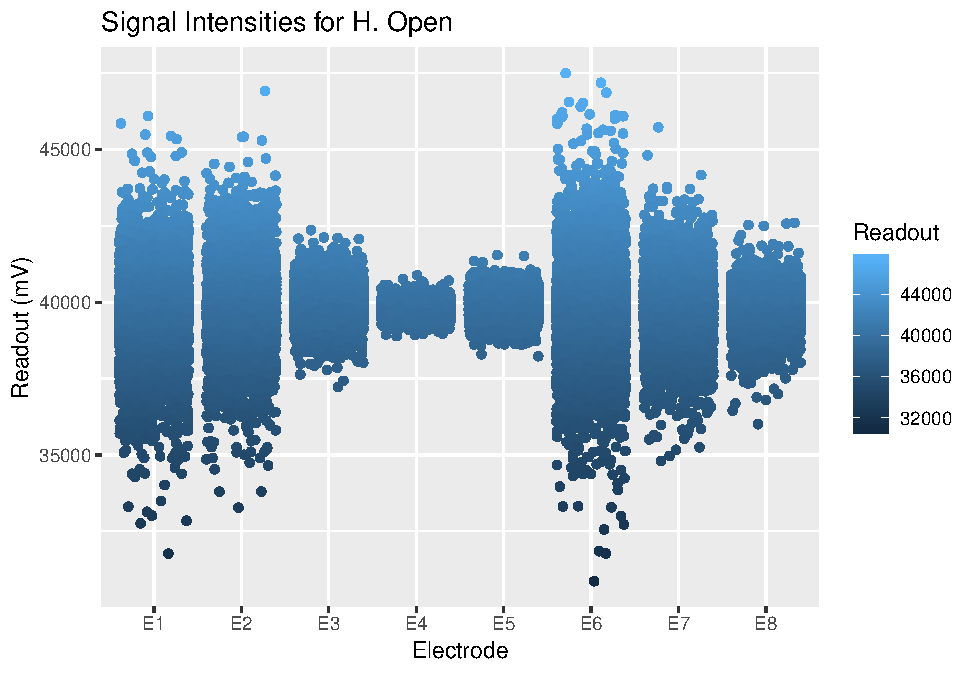
\includegraphics{Megahand_files/figure-latex/unnamed-chunk-5-3.pdf}

\begin{verbatim}
## 
## [[4]]
\end{verbatim}

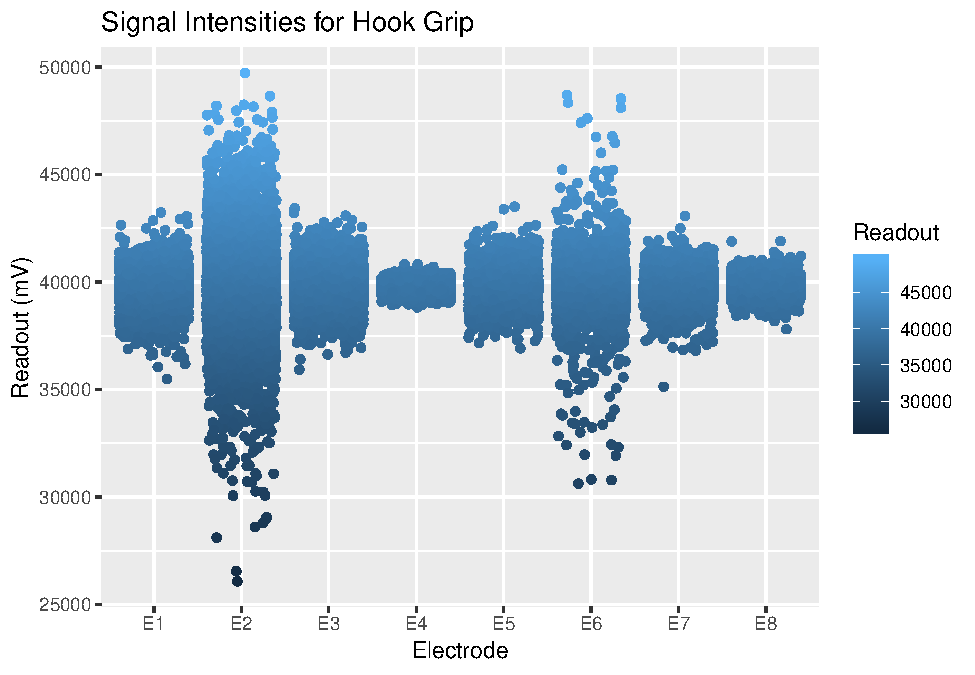
\includegraphics{Megahand_files/figure-latex/unnamed-chunk-5-4.pdf}

\begin{verbatim}
## 
## [[5]]
\end{verbatim}

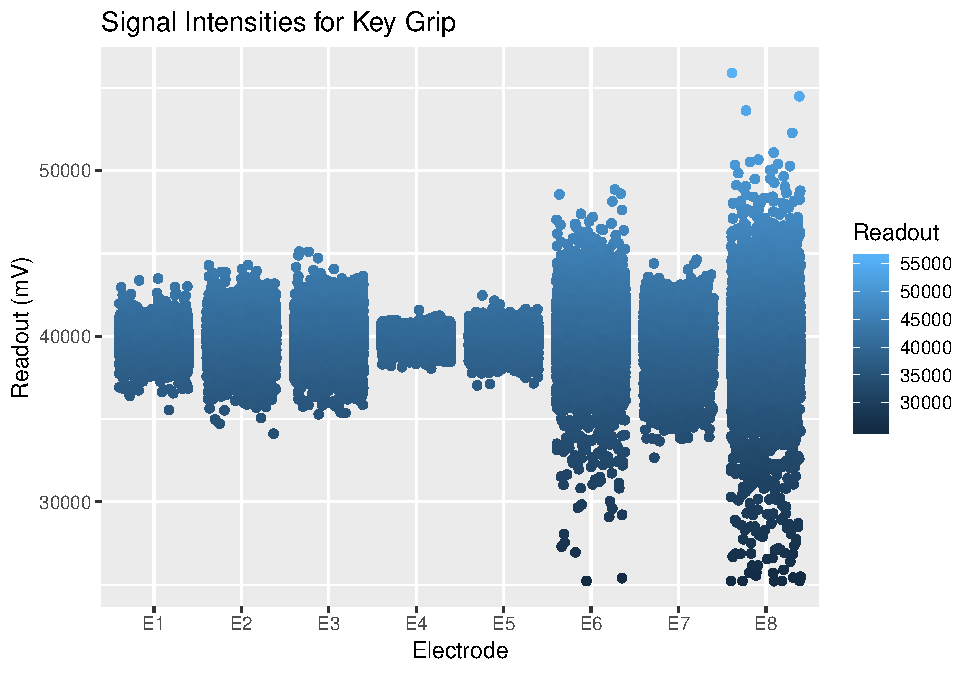
\includegraphics{Megahand_files/figure-latex/unnamed-chunk-5-5.pdf}

\begin{verbatim}
## 
## [[6]]
\end{verbatim}

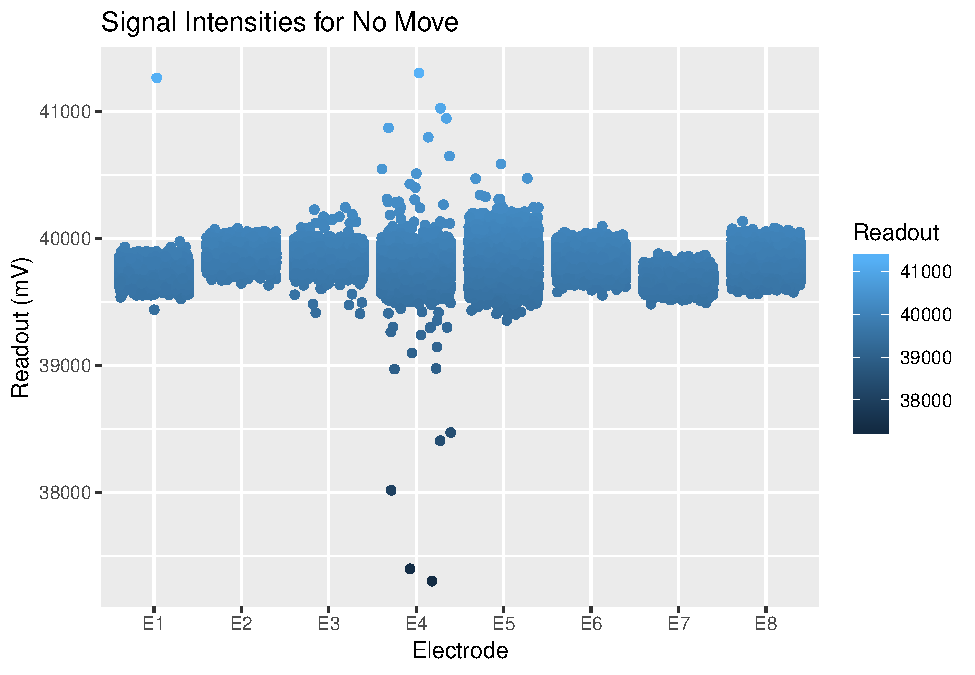
\includegraphics{Megahand_files/figure-latex/unnamed-chunk-5-6.pdf}

\begin{verbatim}
## 
## [[7]]
\end{verbatim}

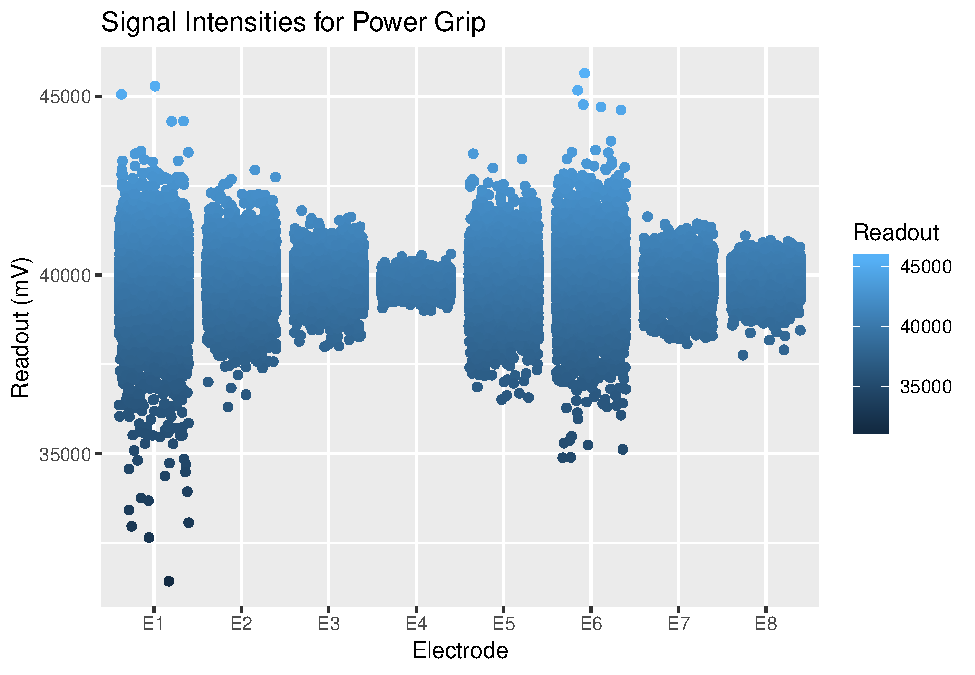
\includegraphics{Megahand_files/figure-latex/unnamed-chunk-5-7.pdf}

\begin{verbatim}
## 
## [[8]]
\end{verbatim}

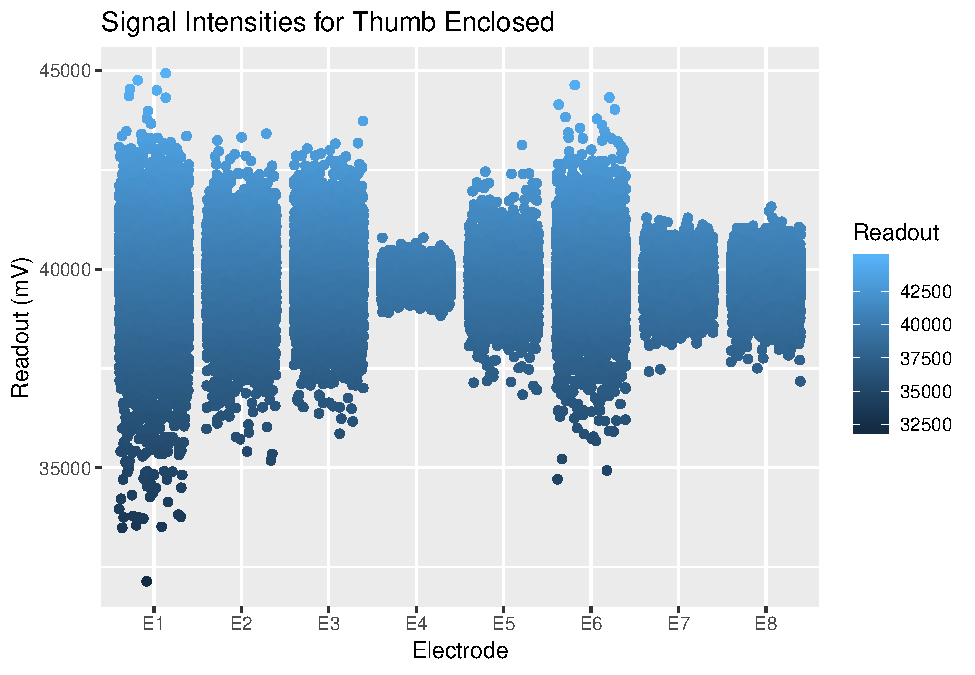
\includegraphics{Megahand_files/figure-latex/unnamed-chunk-5-8.pdf}

\begin{verbatim}
## 
## [[9]]
\end{verbatim}

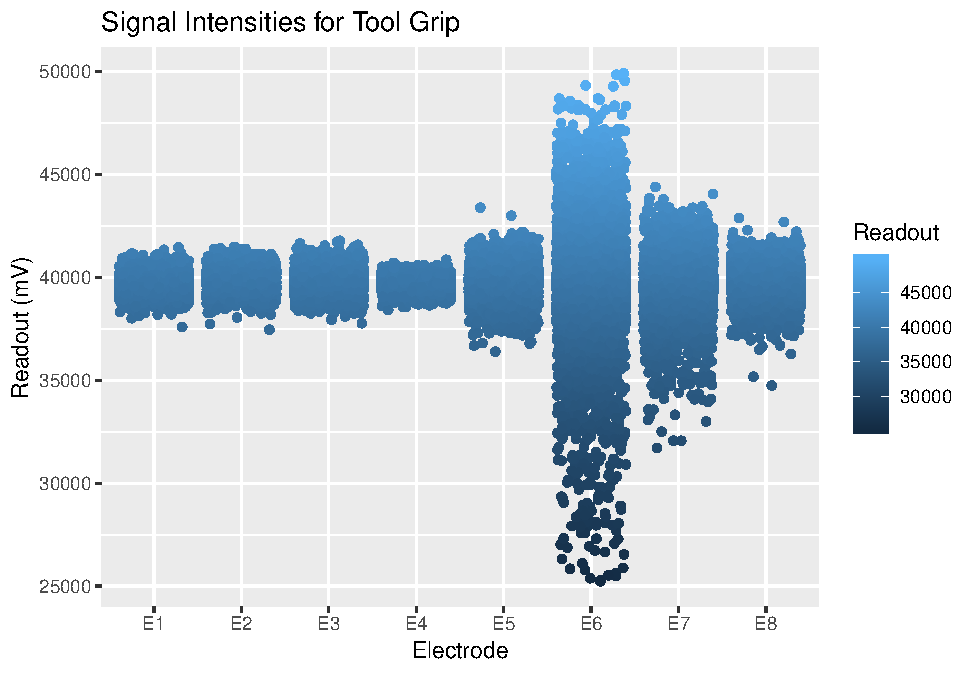
\includegraphics{Megahand_files/figure-latex/unnamed-chunk-5-9.pdf}

\begin{verbatim}
## 
## [[10]]
\end{verbatim}

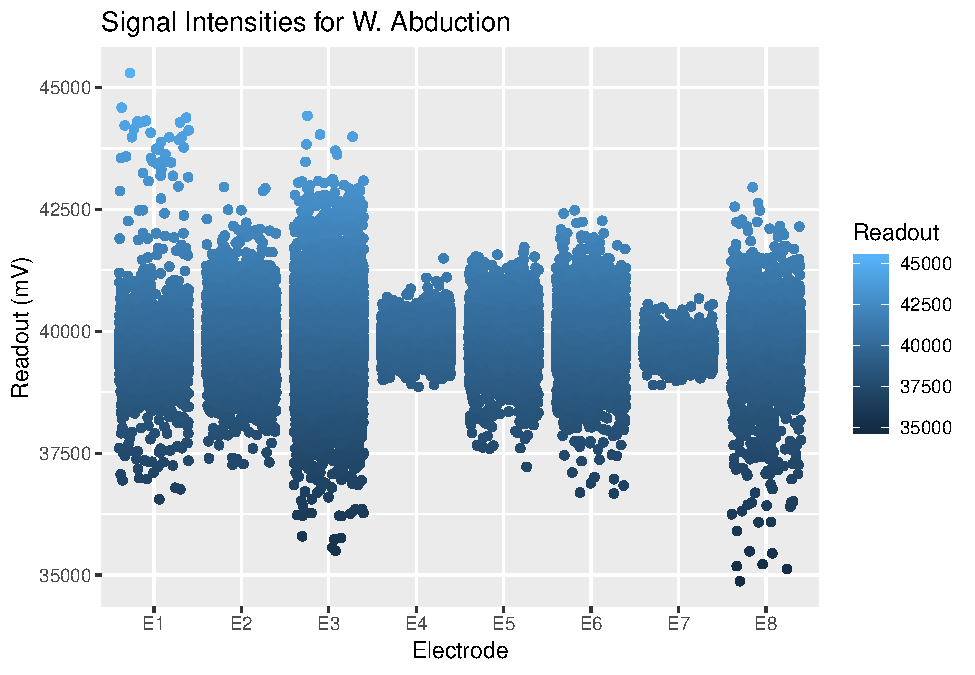
\includegraphics{Megahand_files/figure-latex/unnamed-chunk-5-10.pdf}

\begin{verbatim}
## 
## [[11]]
\end{verbatim}

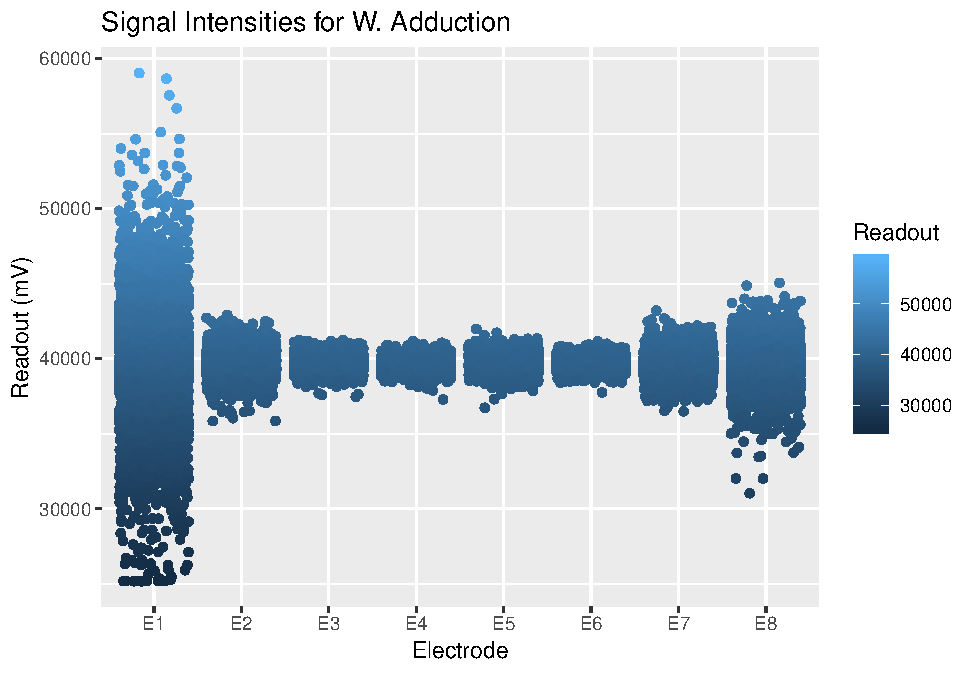
\includegraphics{Megahand_files/figure-latex/unnamed-chunk-5-11.pdf}

\begin{verbatim}
## 
## [[12]]
\end{verbatim}

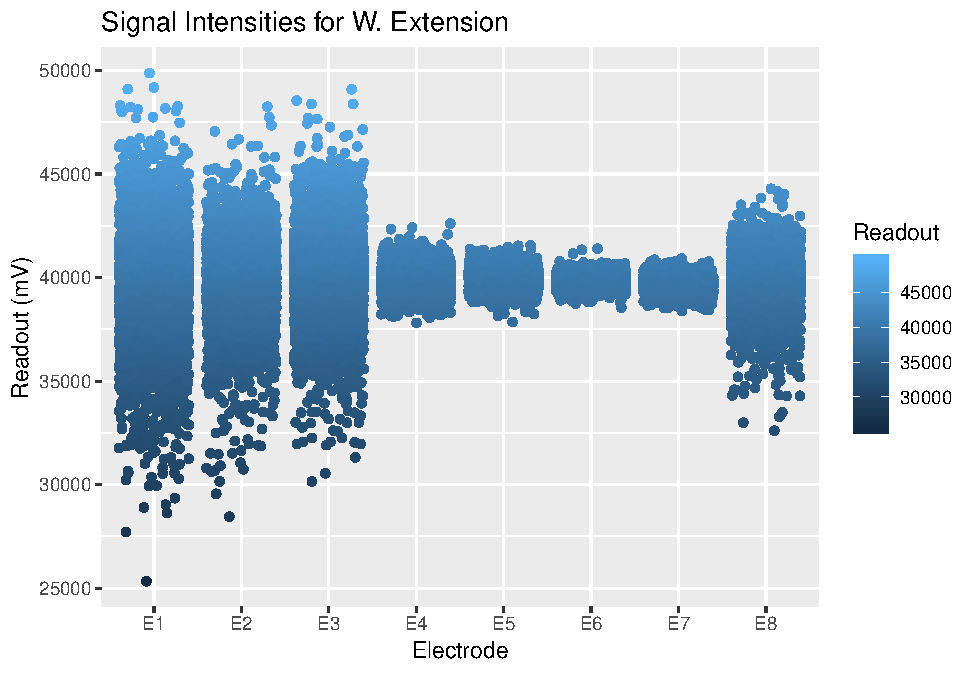
\includegraphics{Megahand_files/figure-latex/unnamed-chunk-5-12.pdf}

\begin{verbatim}
## 
## [[13]]
\end{verbatim}

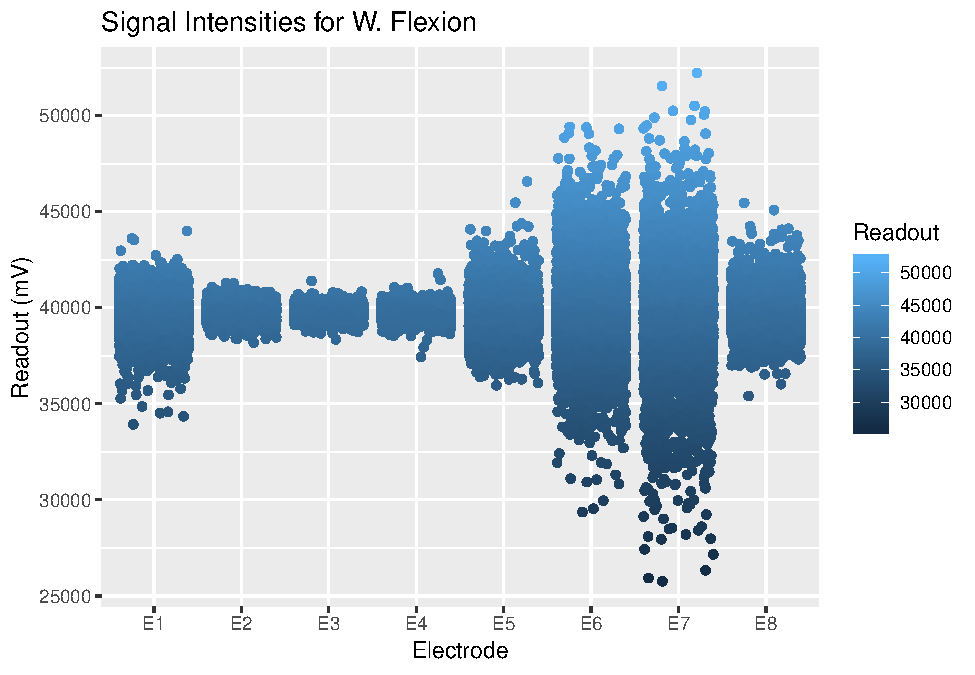
\includegraphics{Megahand_files/figure-latex/unnamed-chunk-5-13.pdf}

\begin{verbatim}
## 
## [[14]]
\end{verbatim}

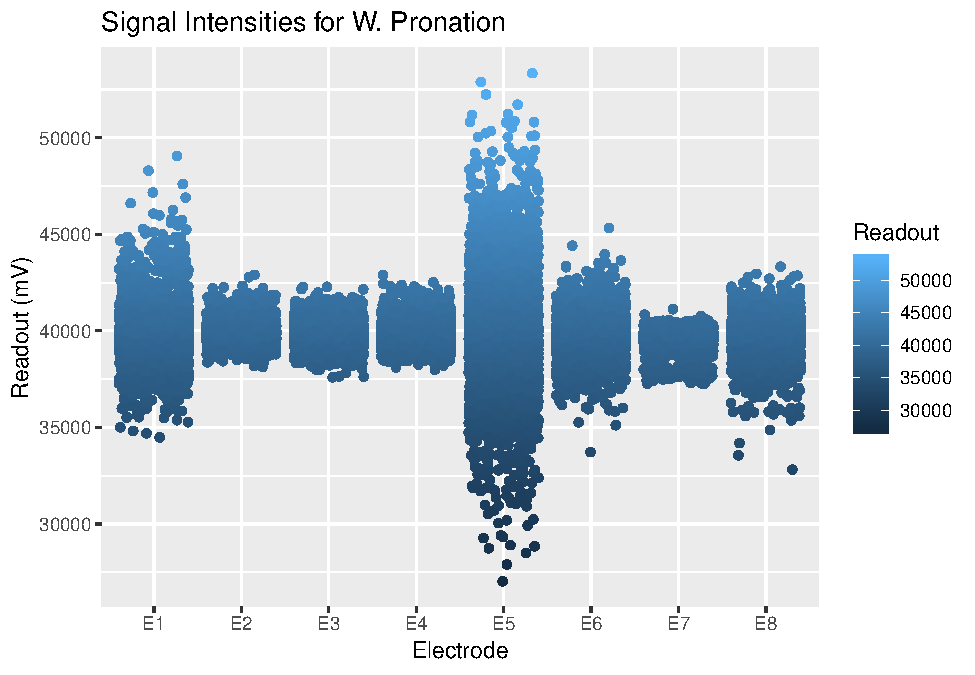
\includegraphics{Megahand_files/figure-latex/unnamed-chunk-5-14.pdf}

\begin{verbatim}
## 
## [[15]]
\end{verbatim}

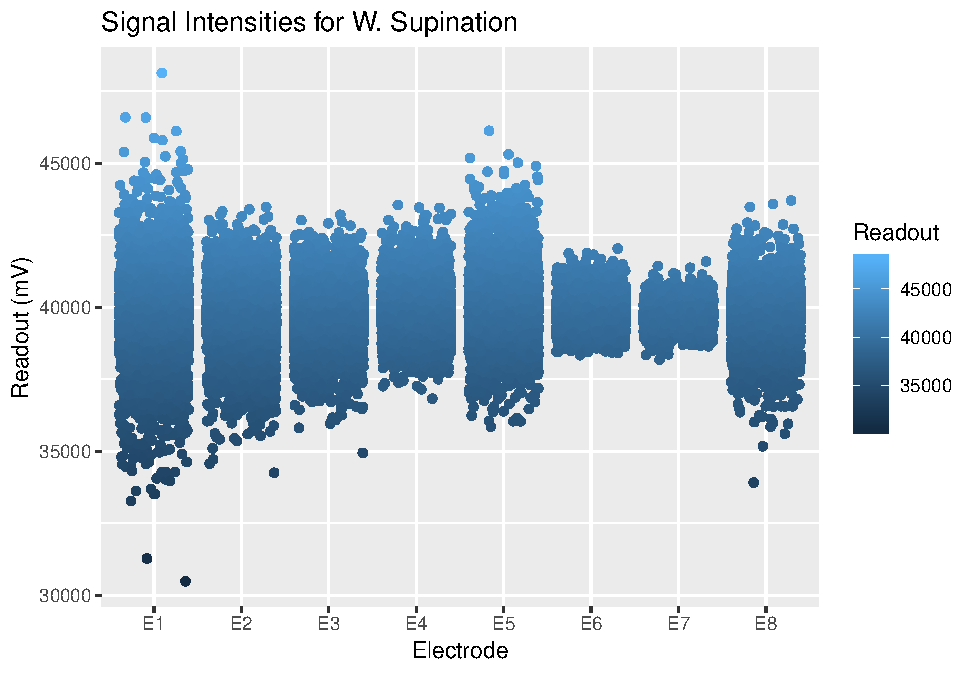
\includegraphics{Megahand_files/figure-latex/unnamed-chunk-5-15.pdf}

\section{Machine Learning}\label{machine-learning}

\begin{Shaded}
\begin{Highlighting}[]
\KeywordTok{install.packages}\NormalTok{(}\StringTok{"tensorflow"}\NormalTok{, }\DataTypeTok{dependencies =} \OtherTok{TRUE}\NormalTok{)}
\KeywordTok{install.packages}\NormalTok{(}\StringTok{"keras"}\NormalTok{, }\DataTypeTok{dependencies =} \OtherTok{TRUE}\NormalTok{)}
\KeywordTok{library}\NormalTok{(tensorflow)}
\KeywordTok{library}\NormalTok{(keras)}
\end{Highlighting}
\end{Shaded}


\end{document}
